\documentclass{beamer}
\usepackage[T1]{fontenc}
\usepackage[utf8]{inputenc}
\usepackage{lmodern}
\usepackage[ngerman]{babel}

\usepackage{graphics}

\usepackage{amsmath}
\usepackage{booktabs}

\usepackage{dot2texi}
\usepackage{tikz}
\usetikzlibrary{arrows,shapes}
\usetikzlibrary{automata}

\usetheme{Singapore}
\usecolortheme{dove}
\graphicspath{{images/}{../comics/}}

\newcommand{\hiddencell}[2]{\action<#1->{#2}}

\AtBeginSection[]
{
  \begin{frame}[plain]
    \frametitle{}
    {\footnotesize
      \tableofcontents[currentsection]
    }
  \end{frame}
}

\title{Grundbegriffe der Informatik}
\author{Patrick Niklaus}

\begin{document}
\begin{frame}
  \frametitle{Grundbegriffe der Informatik}
  \framesubtitle{5. Tutorium}
  \begin{description}
    \item \textbf{Name:} Patrick Niklaus
    \item \textbf{E-Mail:} patrick.niklaus@student.kit.edu
    \item \textbf{Nr:} 43
  \end{description}
\end{frame}

\section{Übungsblatt}
\begin{frame}
  \frametitle{Anmerkungen zum letzten Übungsblatt}
  \begin{enumerate}
    \item Ein Ableitungsbaum beinhaltet in jedem Knoten genau ein Symbol.
    \item Als Startsymbol bei einer Grammatik, verwendet man genau ein Symbol.
    \item Wenn man schreiben will "'w lässt sich von der Grammatik G erzeugen"' kann man schreiben:
      \begin{description}
        \item[$w \in L(G)$:] w ist in der Sprache die G erzeugt. ($w \in T^*$)
        \item[$S \Longrightarrow^* w$:] w lässt sich in beliebig vielen Schritten ableiten.
        \item[$S \Longrightarrow^n w$:] w lässt sich in n Schritten ableiten.
      \end{description}
    \item L(G) enthält nur Wörter aus \emph{Terminalsymbolen}.
  \end{enumerate}
\end{frame}


\section{Motivation Graphen}
\begin{frame}[fragile]
  \frametitle{Was ist ein Graph?}
  \begin{figure}
    \begin{minipage}{5cm}
      \begin{tikzpicture}[->,>=stealth',shorten >=1pt,auto,node distance=2.8cm,
                          semithick]
        \begin{dot2tex}[styleonly,codeonly,neato]
          digraph G {
            d2ttikzedgelabels = true;
            node [style="state"];
            edge [style="-to",topath="bend left"];
            A -> B
            B -> B [topath="loop above"]
            B -> C
            C -> B
            C -> A
          }
        \end{dot2tex}
      \end{tikzpicture}
    \end{minipage}
    \begin{minipage}{5cm}
      \begin{tikzpicture}[auto,node distance=2.0cm, semithick]
        \begin{dot2tex}[styleonly,codeonly,neato]
          graph G {
            d2ttikzedgelabels = true;
            node [style="state"];
            edge [];
            A -- B
            B -- C
            B -- D
          }
        \end{dot2tex}
      \end{tikzpicture}
    \end{minipage}
  \end{figure}
\end{frame}

\section{Gerichtete Graphen}
\subsection{Definitionen}
\begin{frame}
  \frametitle{Gerichtete Graphen}
  \begin{definition}
    \begin{description}
      \item[V:] Menge von Knoten
      \item[$E \subseteq V \times V$:] Menge von Kanten
    \end{description}
    Dann heißt der Tupel G := (V, E) ein gerichteter \emph{Graph}.
  \end{definition}
\end{frame}
\begin{frame}
	\frametitle{Wichtige Begriffe}
	\begin{definition}
    Sei $G = (V, E)$ ein Graph und $x, y \in V$.
		\begin{description}
			\item[x und y sind adjazent:] \hfill \\
        Es gibt eine Kante $(x,y)\in E$.\pause
			\item[Schlinge:] \hfill \\
        Eine Kante der Form $(x,x)\in E$.\pause
			\item[Schlingenfrei:] \hfill \\
        Ein Graph besitzt keine Schlingen.\pause
			\item[Teilgraph:] \hfill \\
        Ein Graph $G'=(V',E')$ mit $V'\subseteq V$ und $E'\subseteq E \cap V'\times V'$.
		\end{description}
	\end{definition}
\end{frame}
\begin{frame}[fragile]
  \frametitle{Beispiele}
  \begin{exampleblock}{}
    \begin{enumerate}
      \item $G_1 := (\{0, 1, 2, 3\}, \{(0, 0), (0, 1), (1, 2), (2, 1)\})$
      \item $G_2 := (\{0, 1, 2, 3\}, \{(0, 2), (3, 1), (2, 1)\})$
    \end{enumerate}
  \end{exampleblock}
  \begin{figure}
    \begin{minipage}{5cm}
      \begin{tikzpicture}[->,>=stealth',shorten >=1pt, auto, semithick, scale=.50]
        \begin{dot2tex}[styleonly,codeonly,neato]
          digraph G {
            d2ttikzedgelabels = true;
            node [style="state"];
            edge [style="-to",topath="bend left"];
            1 -> 2
            2 -> 1;
            0 -> 1
            0 -> 0 [topath="loop below"]
            3;
          }
        \end{dot2tex}
      \end{tikzpicture}
      \caption{$G_1$}
    \end{minipage}
    \begin{minipage}{5cm}
      \begin{tikzpicture}[->,>=stealth',shorten >=1pt, auto, semithick, scale=.75]
        \begin{dot2tex}[styleonly,codeonly,neato]
          digraph G {
            d2ttikzedgelabels = true;
            node [style="state"];
            edge [style="-to",topath="bend left"];
            0 -> 2
            3 -> 2
            1 -> 2
            1 -> 3
          }
        \end{dot2tex}
      \end{tikzpicture}
      \caption{$G_2$}
    \end{minipage}
  \end{figure}
\end{frame}

\subsection{Knotengrad}
\begin{frame}
  \frametitle{Knotengrad}
  \begin{definition}
    Sei G = (V, E) ein gerichteter Graph.
    \begin{description}
      \item[Ausgangsgrad:] $d_+(x) := |\{(x, e) \in E | e \in V\}|$
      \item[Eingangsgrad:] $d_-(x) := |\{(e, x) \in E | e \in V\}|$
    \end{description}
  \end{definition}
\end{frame}
\begin{frame}[fragile]
  \frametitle{Welchen Grad haben die Knoten?}
    \begin{figure}
      \begin{tikzpicture}[->,>=stealth',shorten >=1pt, auto, semithick, scale=.75]
        \begin{dot2tex}[styleonly,codeonly,neato]
          digraph G {
            d2ttikzedgelabels = true;
            node [style="state"];
            edge [style="-to",topath="bend left"];
            0 -> 2
            3 -> 2
            1 -> 2
            1 -> 3
          }
        \end{dot2tex}
      \end{tikzpicture}
    \end{figure}
\end{frame}

\subsection{Pfade}
\begin{frame}
	\frametitle{Pfade}
	\begin{block}{Definition}
		Ein Pfad ist eine Liste $p=(v_0, \ldots ,v_n) \in V^+$ mit: $\forall i \in {\mathbb G}_n: (v_i,v_{i+1})\in E$
		\begin{description}
			\item[Länge:]\hfill \\
        Die Anzahl der Kanten $n = |p| - 1$. \pause
			\item[Wiederholungsfrei:] \hfill \\
        Alle Knoten sind je paarweise verschieden, maximal $v_0$ und $v_n$ sind gleich. \pause
			\item[Geschlossen:] \hfill \\
        Wenn gilt $v_0 = v_n$. Der Pfad heißt dann auch \emph{Zyklus}.\pause
			\item[Einfacher Zyklus:] \hfill \\
        Ein geschlossener und wiederholungsfreier Pfad.
    \end{description}
	\end{block}
\end{frame}
\begin{frame}[fragile]
  \frametitle{Welche Pfade gibt es in diesem Graphen?}
    \begin{figure}
      \begin{tikzpicture}[->,>=stealth',shorten >=1pt, auto, semithick, scale=.75]
        \begin{dot2tex}[styleonly,codeonly,neato]
          digraph G {
            d2ttikzedgelabels = true;
            node [style="state"];
            edge [style="-to",topath="bend left"];
            1 -> 2
            2 -> 1;
            0 -> 1
            0 -> 0 [topath="loop below"]
            3;
          }
        \end{dot2tex}
      \end{tikzpicture}
    \end{figure}
\end{frame}

\section{Gerichtete Bäume}
\subsection{Definition}
\begin{frame}
	\frametitle{Gerichtete Bäume}
	\begin{definition}
    Ein gerichteter Graph $G = (V, E)$ heißt \emph{gerichteter Baum} wenn gilt:
		\begin{enumerate}
			\item $\exists r \in V$ mit: $\forall x\in V$ ex. genau ein Pfad von $r$ nach $x$ \pause
			\item Es gibt genau einen solchen Knoten $r$.
		\end{enumerate}
	\end{definition}
\end{frame}
\begin{frame}[fragile]
  \frametitle{Beispiel}
    \begin{figure}
      \begin{tikzpicture}[->,>=stealth',shorten >=1pt, auto, semithick, scale=.75]
        \begin{dot2tex}[styleonly,codeonly,dot]
          digraph G {
            d2ttikzedgelabels = true;
            node [style="state"];
            edge [style="-to"];
            5 -> 3;
            5 -> 7;
            3 -> 2;
            3 -> 4;
            7 -> 6;
            7 -> 9;
          }
        \end{dot2tex}
      \end{tikzpicture}
    \end{figure}
\end{frame}

\section{Ungerichtete Graphen}
\subsection{Definition}
\begin{frame}
  \frametitle{Ungerichtete Graphen}
  \begin{definition}
    \begin{description}
      \item[V:] Menge von Knoten
      \item[$E \subseteq \{\{x, y\} | x, y \in V\}$:] Menge von Kanten
    \end{description}
    Dann heißt der Tupel $U := (V, E)$ ein ungerichteter \emph{Graph}.\\
    Wir nennen $G_U = (V, \{(x, y) | \{x, y\} \in E\})$ den zu U gehörenden gerichteten Graphen.
  \end{definition}
\end{frame}
\begin{frame}[fragile]
	\frametitle{Beispiel}
  \begin{figure}
    \begin{dot2tex}[straightedges,circo]
      graph G {
        mindist = 0.5;
        node [shape="circle"];
        a -- b;
        a -- c;
        a -- d;
        b -- c;
        d -- d;
        d -- c;
      }
    \end{dot2tex}
  \end{figure}
	\only<1->{Wie sähe dieser ungerichtete Graph als Menge aus?\\}
	\only<2->{$G = ( \{a,b,c,d\}, \{\{a,b\},\{a,c\},\{a,d\},\{b,c\},\{d,b\},\{d,c\}\})$}
\end{frame}

\subsection{Wege}
\begin{frame}
	\frametitle{Wege}
	\begin{definition}
		Ein Weg ist eine Liste $p=(v_0, \ldots ,v_n) \in V^+$ mit: $\forall i \in {\mathbb G}_n: \{v_i,v_{i+1}\} \in E$.\\
    Länge, Wiederholungfreiheit, Geschlossenheit sind analog zu Pfaden definiert.
	\end{definition}
\end{frame}
\begin{frame}[fragile]
  \frametitle{Welche Wege gibt es in diesem Graphen?}
    \begin{figure}
      \begin{tikzpicture}[shorten >=1pt, auto, semithick, scale=.5]
        \begin{dot2tex}[styleonly,codeonly,neato]
          graph G {
            d2ttikzedgelabels = true;
            node [style="state"];
            edge [path="bend left"];
            0 -- 2;
            2 -- 3;
            2 -- 6;
            1 -- 4;
            1 -- 5;
          }
        \end{dot2tex}
      \end{tikzpicture}
    \end{figure}
\end{frame}

\begin{frame}
	\frametitle{Zusammenhängende Graphen}
	\begin{definition}
    Sei $G = (V, E)$ ein Graph.
		\begin{description}
			\item[G ist gerichtet:] \hfill \\
			  G heißt \emph{streng zusammenhängend} wenn für jedes Knotenpaar $(x,y)\in V^2$ gilt: Es gibt einen Pfad von $x$ nach $y$.
			\item[G ist ungerichtet:] \hfill \\
        G heißt \emph{zusammenhängend}, wenn der entsprechende gerichtete Graph \emph{streng zusammenhängend} ist.
		\end{description}
	\end{definition}
\end{frame}

\begin{frame}
	\frametitle{Isomorphe Graphen}
	\begin{definition}
    Seien $G_1 = (V_1, E_1), G_2 = (V_2, E_2)$ zwei Graphen.\\
    Wenn eine Bijektion $f: E_1 \rightarrow E_2$ existiert, sodass gilt:\\
    $\{(f(x), f(y)) | (x, y) \in E_1\} = E_2$ heißt $G_1$ zu $G_2$ \emph{isomorph}.
	\end{definition}
\end{frame}

\subsection{Aufgaben}
\begin{frame}[fragile]
  \frametitle{Aufgaben}
  \begin{exampleblock}{}
      Welche der Graphen sind isomorph? Gebt ggf. eine passende Knoten-Bijektion an.
    \begin{figure}
      \begin{minipage}{4cm}
        \begin{tikzpicture}[auto, semithick, scale=.5]
          \begin{dot2tex}[codeonly,twopi]
            graph G {
              d2ttikzedgelabels = true;
              node [shape="circle"];
              edge [];
              0 -- 1;
              0 -- 2;
              0 -- 3;
              0 -- 4;
              1 -- 2;
              1 -- 4;
              2 -- 3;
              3 -- 4;
            }
          \end{dot2tex}
        \end{tikzpicture}
        \caption{$G_1$}
      \end{minipage}
      \begin{minipage}{3cm}
        \begin{tikzpicture}[auto, semithick, scale=.5]
          \begin{dot2tex}[codeonly,neato]
            graph G {
              d2ttikzedgelabels = true;
              node [shape="circle"];
              edge [];
              0 -- 1
              0 -- 2
              0 -- 3
              0 -- 4;
              1 -- 2 -- 3 -- 4;
            }
          \end{dot2tex}
        \end{tikzpicture}
        \caption{$G_2$}
      \end{minipage}
      \begin{minipage}{3cm}
        \begin{tikzpicture}[auto, semithick, scale=.5]
          \begin{dot2tex}[codeonly,circo]
            graph G {
              d2ttikzedgelabels = true;
              node [shape="circle"];
              edge [];
              2 -- 5;
              2 -- 0;
              2 -- 3;
              2 -- 4;
              5 -- 0;
              5 -- 3;
              0 -- 4;
              3 -- 4;
            }
          \end{dot2tex}
        \end{tikzpicture}
        \caption{$G_2$}
      \end{minipage}
    \end{figure}
  \end{exampleblock}
\end{frame}


\section{Abschluss}
\subsection{Zusammenfassung}
\begin{frame}
  \frametitle{Was ihr jetzt wissen sollte.}
  \begin{enumerate}
    \item Wie ist ein gerichteter Graph definiert?
    \item Wie ist ein ungerichteter Graph definiert?
    \item Was ist ein Pfad/Weg?
    \item Was sind Schleifen?
    \item Was ist ein zusammenhängender Graph?
    \item Was ist ein Baum?
    \item Wie sieht der zu einem ungerichteten Graphen gehörende gerichtete Graph aus?
  \end{enumerate}
\end{frame}

\subsection{xkcd}
\begin{frame}[plain]
  \begin{figure}
    \begin{center}
      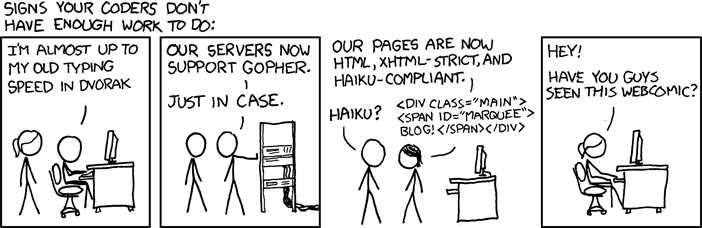
\includegraphics[width=320pt]{not_enough_work}
    \end{center}
  \end{figure}
  {\tiny It's even harder if you are an asshole who pronounces <> brackets.}
\end{frame}

\end{document}
